% ---
% tags: [LLM, 推理优化, PD分离]
% author: marshall
% excerpt:
% ---
\documentclass[11pt]{article}

\usepackage{fontspec}
\usepackage{xeCJK}
% macOS 上 SimSun 位于 Microsoft Word 内部；如需其它字体请修改下面路径
\setCJKmainfont[Path=/Applications/Microsoft Word.app/Contents/Resources/DFonts/, Extension=.ttc]{Simsun}

\usepackage[a4paper, margin=2.2cm]{geometry}
\linespread{1.3}
\setlength{\parskip}{0.3em}
\usepackage{amsmath, amssymb, amsthm}
\usepackage{graphicx}
% 本文图片统一放在与 .tex 同名的文件夹 latex/<slug>/ 中，直接用文件名引用即可
\graphicspath{{./}{2026-11-23-pd-disaggregation/}}
\usepackage{hyperref}
\hypersetup{colorlinks=true, linkcolor=blue, urlcolor=blue}

\title{做 PD 分离时，我们到底在做些什么}
\author{Marshall}

\begin{document}
\maketitle

\section{初识 PD 分离}

众所周知，大模型的推理分为两个环节：

\begin{itemize}
  \item Prefill：对输入序列进行一次完整的模型前向（forward）计算，产出第一个 Token 以及输入序列的 KV Cache；
  \item Decode：利用 Prefill 阶段产生的 KV Cache，重复进行多次模型的前向，自回归产出新的 Token 作为模型的输出。
\end{itemize}

我们深入一点来分析，就可以知道这两个阶段的计算负载完全是两种情况：

\begin{itemize}
  \item 对于 Prefill 阶段，输入的序列往往是很长的，其与模型权重进行的计算一般是矩阵乘（GEMM），也就是说 Prefill 阶段对于计算单元需求比较高，换句话说，\textbf{Prefill 是计算受限（compute bound）的}。
  \item 对于 Decode 阶段，每次模型前向只需要处理一个新的 Token（qkv 中的 q 长度为 1），因此其与模型权重进行的计算一般是矩阵向量乘（GEMV）。由于每生成一个 Token 都需要反复读取模型权重，同时还要访问历史 KV Cache，因此需要数据在存储单元之间反复的运输，其对于带宽的需求比较高，换句话说，\textbf{Decode 是访存受限（memory bound）的}。
\end{itemize}

那么，一个自然而然的想法就是：既然两种负载对硬件的需求不同，我们能不能把它们放到不同类型的机器上运行？例如，让计算能力更强的 NPU/GPU 集群负责 Prefill，作为 P 节点；让显存带宽和显存容量更适合 Decode 负载的 GPU 集群负责 Decode，作为 D 节点。

这样一来，两种硬件就可以各司其职，\textbf{让不同阶段的计算负载与硬件资源更加匹配}，从而提高整个推理集群的资源利用率和吞吐能力。这就是 PD Disaggregation（Prefill--Decode Disaggregation），也就是我们常说的 PD 分离。

\section{异构机器分离真的足够了吗？}

上面讲的是一种比较直观的想法，但\textbf{PD 分离的价值，真的只是让不同类型的硬件各司其职吗？}

其实很多时候我们的硬件资源并不那么理想，大部分时候我们还是只有一种硬件资源，甚至于没那么多机器，可能就只有一个节点 8 张卡，那么这时候我们做 PD 分离还有什么意义呢？

让我们再往下深入看一层，我们知道真实的 server 场景中，输入 request 的长短是极端不均衡的，有些请求只有几十个 Token，有些请求却可能有几万甚至几十万 Token。

\begin{figure}[htbp]
  \centering
  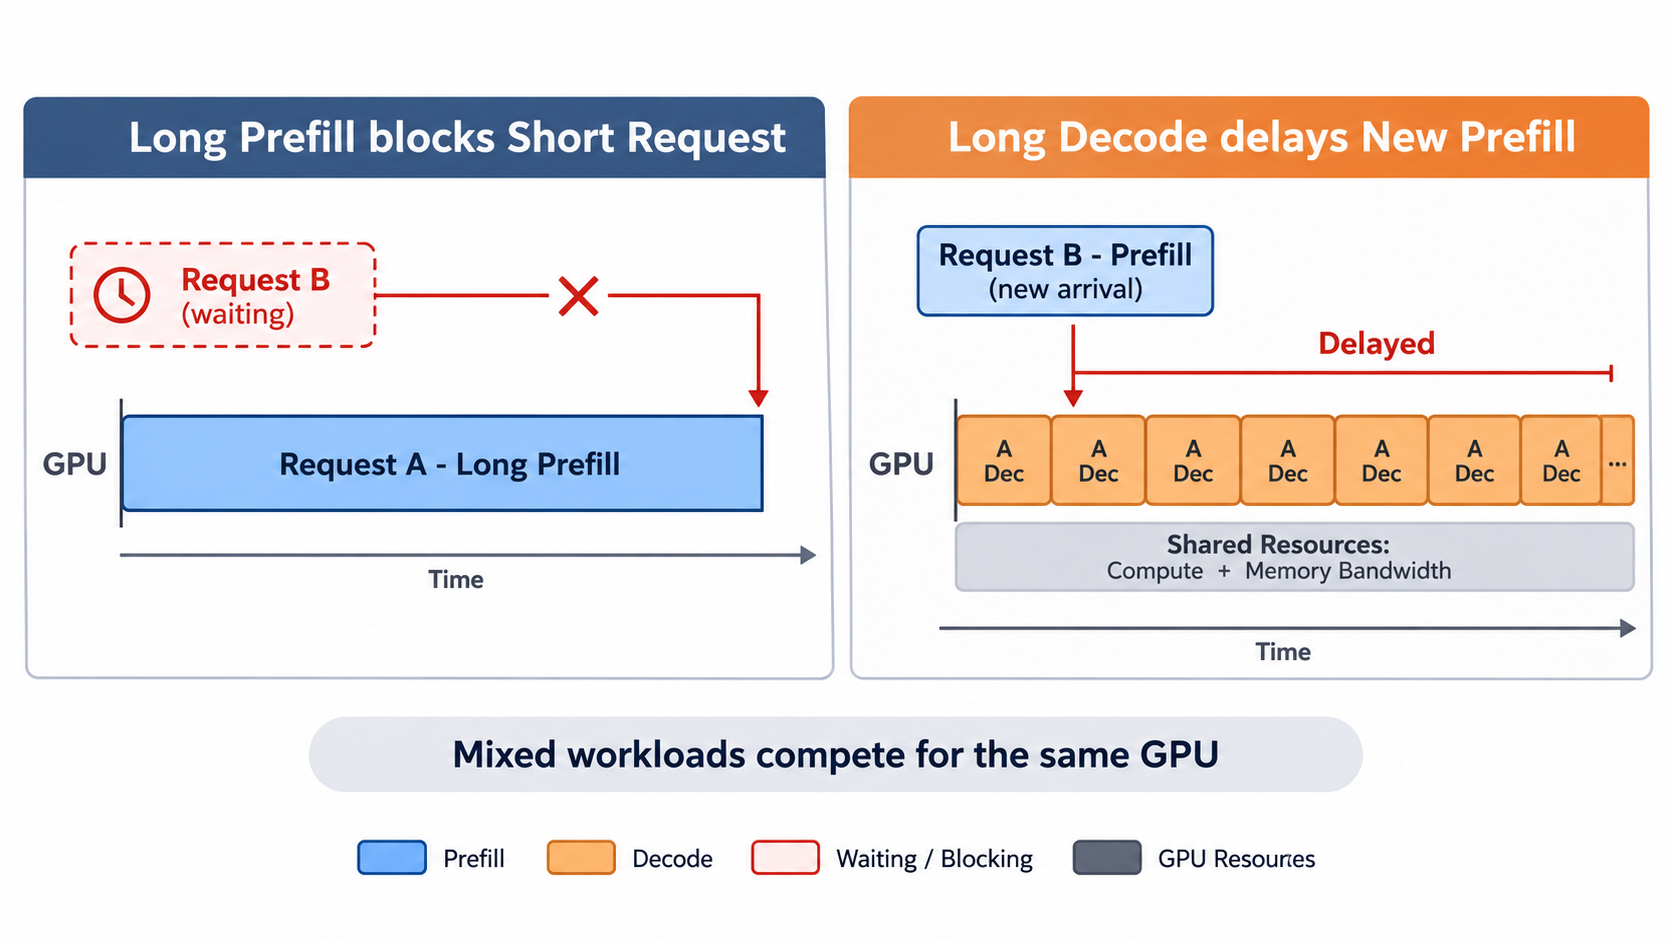
\includegraphics[width=0.9\textwidth]{fig-queue.png}
  \caption{输入请求长短不均衡：短请求 B 排在超长请求 A 之后，需要等待 A 的 Prefill 完成才能获得计算资源}
  \label{fig:queue}
\end{figure}

假设现在有一个很短的 Request B，排在一个超长的 Request A 后面，那么 B 就可能需要等待 A 的 Prefill 完成，才能获得计算资源。反过来，如果 A 已经进入 Decode 阶段，但它需要生成很长的输出，那么新到来的 Request B 也可能因为资源竞争而无法及时进行 Prefill。

当然，现代推理框架已经针对这些问题做了不少优化。例如：

\begin{itemize}
  \item Continuous Batching：不再等一个批次（batch）内所有请求一起完成，而是在每个 Decode 结束后动态加入和移除请求，让计算资源尽可能持续地被利用。
  \item Chunked Prefill：将一个很长的 Prefill 请求切分成多个 Chunk，分批执行，避免一个超长 Prompt 长时间独占 GPU，影响其他请求的 Decode。
\end{itemize}

这些优化确实缓解了请求之间的资源竞争，但它们并没有从根本上消除 Prefill 和 Decode 之间的计算干扰。

\textbf{我们考虑一个 PD 未分离的场景：}

假设当前有一批 Request 正在进行 Decode，调度器发现此时有一个新的 Prefill 请求需要处理，于是决定将一部分 GPU 计算资源分配给这个 Prefill。这其实不是一件太愉快的事情：Prefill 和 Decode 虽然都在同一张 GPU 上运行，但它们的资源需求其实是完全不同的。Prefill 需要大量计算资源，会产生较大的 GEMM 负载；Decode 则需要频繁读取模型权重和 KV Cache，对显存带宽有较高要求。当两者同时执行时，就可能出现计算单元、显存带宽、缓存、SM、调度资源等方面的竞争。因此一次 Prefill 的介入，就可能导致 Decode 的 TPOT 出现明显抖动。

\textbf{当 PD 分离的时候：}

我们不再让 Prefill 和 Decode 争抢同一组 GPU 计算资源，而是将它们放到不同的 GPU 实例上。这样一来，调度器可以独立地决定哪些请求进入 Prefill，哪些请求进入 Decode，而不会因为一个新的 Prefill 请求到来，就直接干扰正在执行的 Decode 负载。

这里，PD 分离真正做的是从资源隔离的角度，将两种不同特征的负载解耦。因此，即使我们没有异构硬件，只有同一种 GPU，甚至只有一个节点，也依然可以考虑 PD 分离。

\section{一个模型，两套 forward}

上面我们所讨论的都是硬件层面的 PD 分离，实际上模型跑的还是同一套 forward。更进一步，我们能否考虑为两种不同的计算负载设计两套不一样的模型 forward 呢？答案当然是可以的。

最直接的就是 Kernel 的分离，因为算子对于输入 tensor 的形状极端敏感，对于 prefill 来说是矩阵乘负载，这时候，我们更关注计算吞吐、矩阵乘效率以及大规模算子的融合。对于 decode 来说是 seq\_len=1 的矩阵向量乘负载，此时，计算规模变小，访存开销在整体执行时间中的占比变得更高。最直观的例子就是 FlashAttention 和 FlashDecoding。

\begin{itemize}
  \item FlashAttention：主要针对 Prefill 中较长的 Q 和 KV 序列，采用分块计算、在线 Softmax 等技术，减少 HBM 与片上存储之间的数据搬运。
  \item FlashDecoding：针对 Decode 中 Q 序列长度较短、KV 序列较长的场景，通过对 KV 序列进行切分和并行计算，再对局部结果进行合并，从而提高 GPU 的并行度。
\end{itemize}

进一步来说，我们甚至可以把这种思想扩展到整个模型 Forward。在 Prefill 路径中，我们可以采用更适合大 Batch、大 Sequence 的算子实现；在 Decode 路径中，则采用更适合低 Batch、低 Q Length 的实现。两条路径在数学语义上保持一致，但底层的 Kernel、融合策略、数据布局，甚至部分计算图都可以不同。

再进一步，如果模型架构本身就考虑了 Prefill 和 Decode 的不同需求，那么还可以在模型结构层面进行优化。

例如，DeepSeek 等模型架构探索中涉及的 Prefill/Decode 非对称计算设计，就体现了这种思路：不再要求两个阶段必须使用完全相同的计算路径，而是针对不同阶段的需求设计不同的计算机制。

\begin{figure}[htbp]
  \centering
  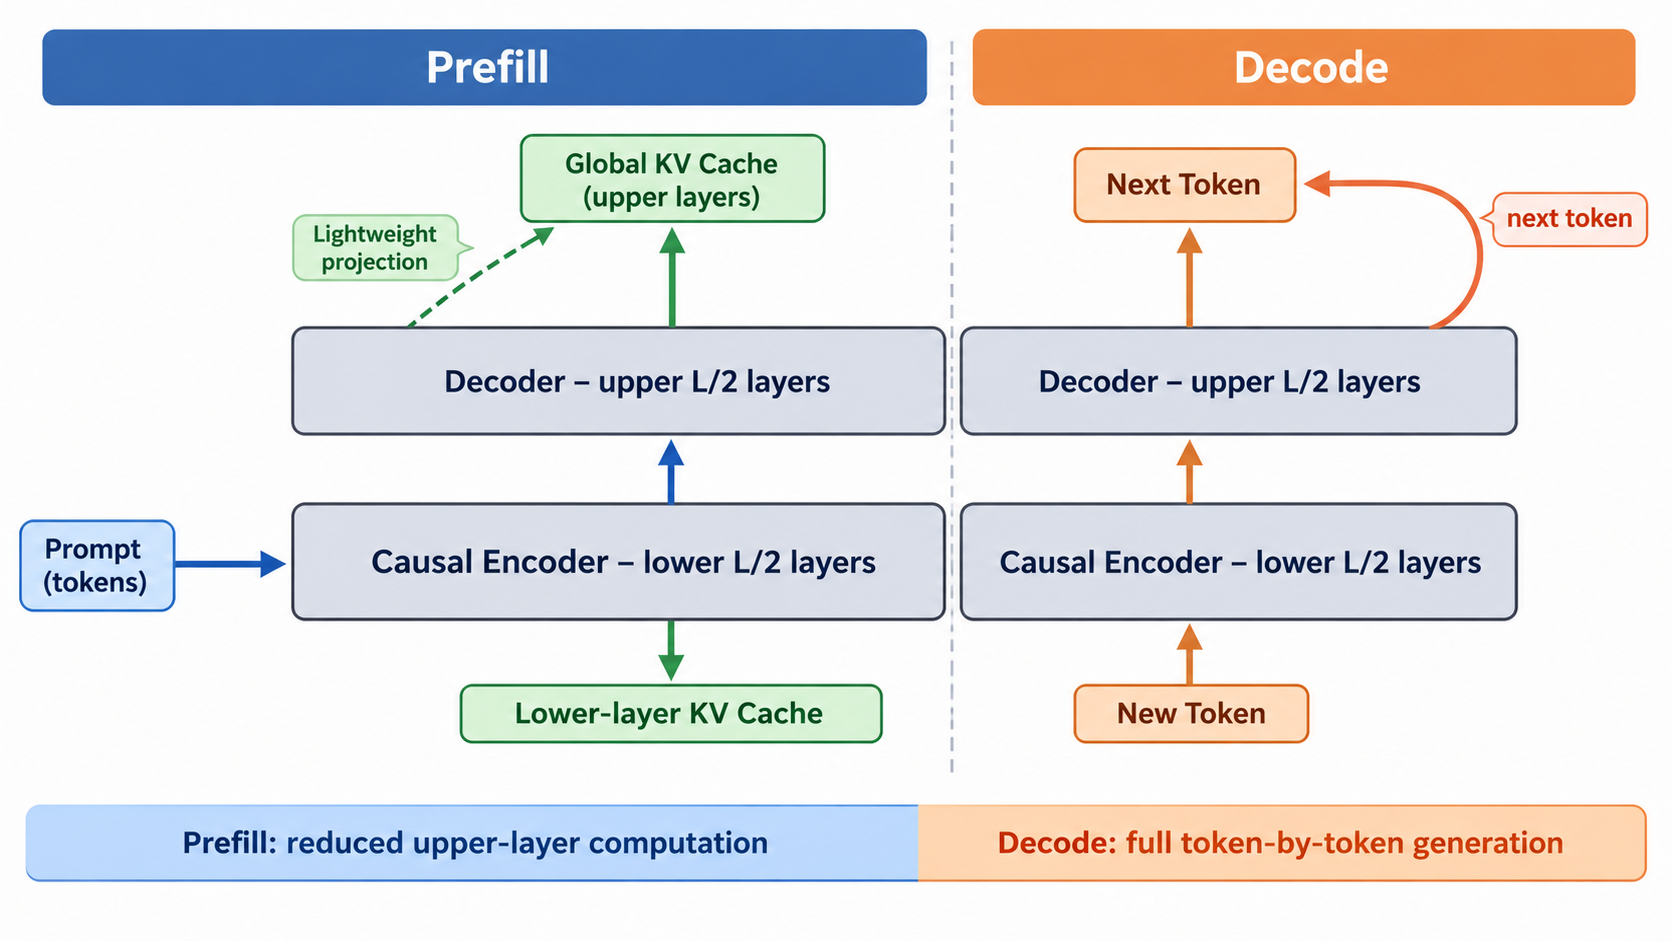
\includegraphics[width=0.9\textwidth]{fig-model.png}
  \caption{模型架构层面的 Prefill/Decode 非对称计算设计}
  \label{fig:model}
\end{figure}

这四种思路，其实正好对应 PD 分离的四个优化层次：

\begin{enumerate}
  \item \textbf{硬件层}：将 Prefill 和 Decode 放到不同的 GPU 或计算节点上。
  \item \textbf{调度层}：让两种负载拥有独立的资源池和调度策略。
  \item \textbf{Kernel 层}：针对不同阶段设计不同的算子实现。
  \item \textbf{模型层}：从模型架构和计算图层面进一步实现 Prefill/Decode 非对称化。
\end{enumerate}

\begin{figure}[htbp]
  \centering
  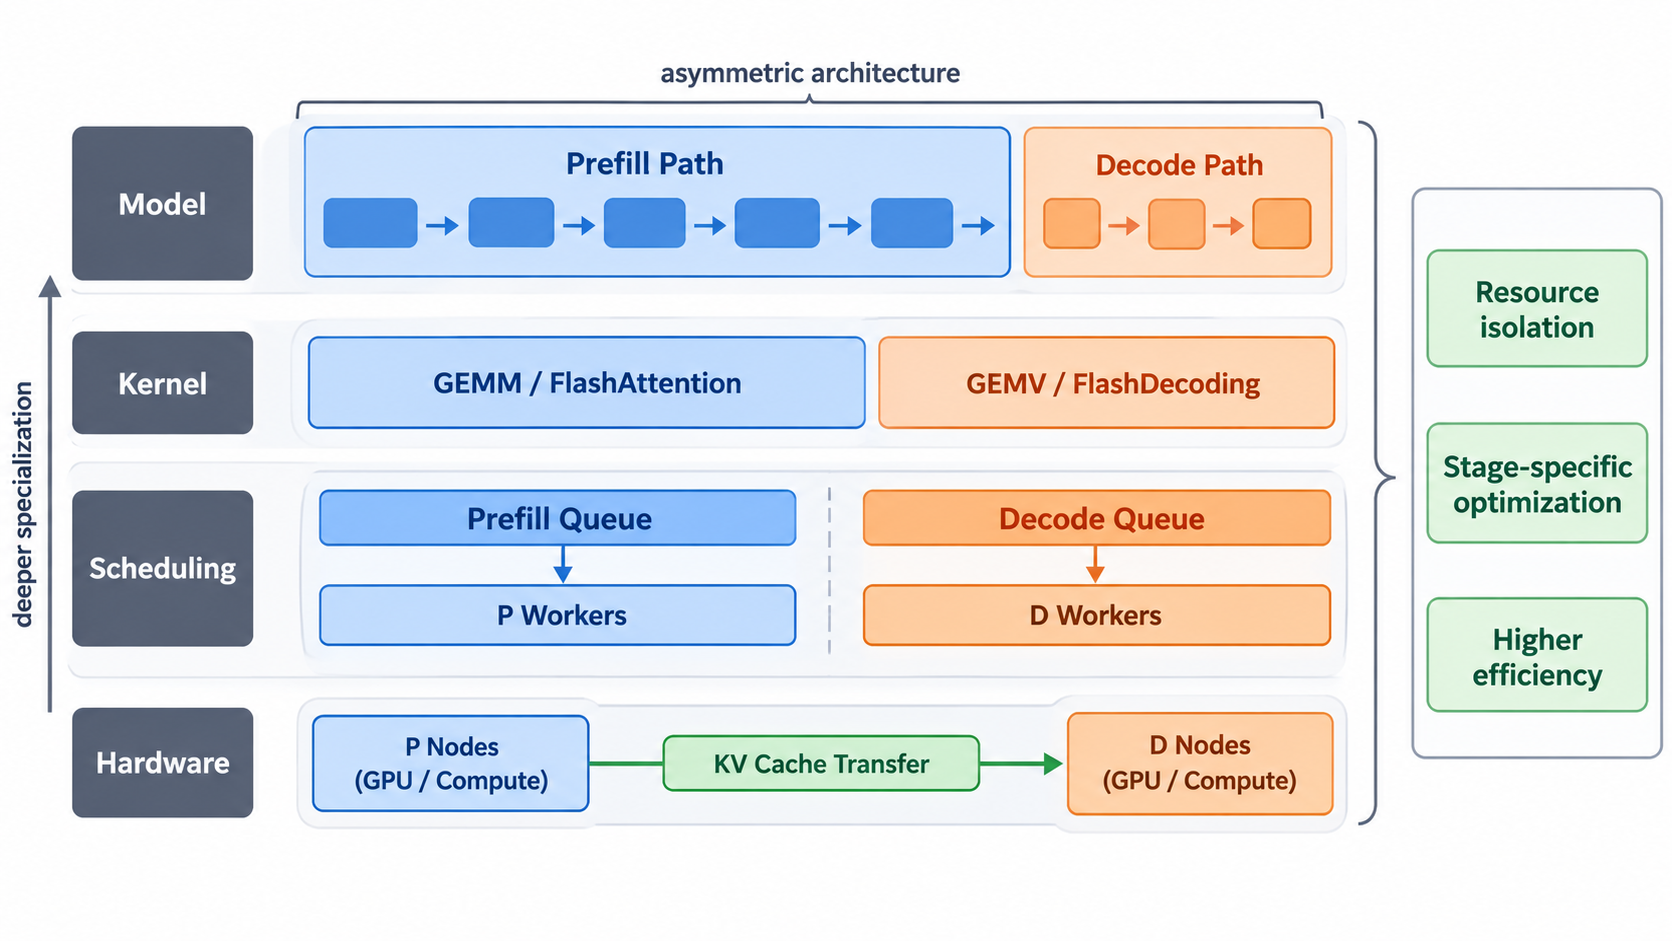
\includegraphics[width=0.9\textwidth]{fig-levels.png}
  \caption{PD 分离的四个优化层次}
  \label{fig:levels}
\end{figure}

\section{葵花宝典：PD 分离配比}

前面我们讨论了 PD 分离的动机，也知道了它可以从硬件、调度、Kernel 甚至模型架构等多个层次进行优化。

但是具体该怎么配 PD 分离的比例呢？给我们一个集群，该配几台 P 几台 D？更进一步，我们选择怎么样的并行方式，P 节点要配多少 TP/DP、D 节点要配多少 TP/DP？这里其实涉及一个非常重要的概念：\textbf{PD 之间的负载均衡（Load Balancing）}。

\subsection{把 PD 分离看成一条流水线}

一个请求首先进入 P 节点，完成 Prefill，生成 KV Cache；随后，KV Cache 被传输到 D 节点，由 D 节点继续完成 Decode，直到请求结束。

也就是说，P 和 D 之间存在明确的生产者—消费者关系：

\begin{itemize}
  \item P 节点负责生产已经完成 Prefill 的请求及其 KV Cache。
  \item D 节点负责消费这些请求，并持续完成 Token 生成。
\end{itemize}

那么问题就来了：如果 P 节点处理请求的速度远远快于 D 节点，会发生什么？

假设 P 节点每秒可以处理 100 个请求，但 D 节点每秒只能完成 50 个请求的 Prefill 接收和后续 Decode 服务，那么随着时间推移，越来越多的请求就会堆积在 P 到 D 的交接位置。反过来，如果 D 节点的处理能力远远大于 P 节点，那么 D 节点就会经常处于空闲状态，等待新的请求完成 Prefill。这两种情况都不是我们希望看到的。因此，我们需要尽可能让 P 和 D 的处理能力相匹配，让整条流水线保持稳定。

\subsection{最基础的 PD 配比估算}

我们先做一个简化假设：

\begin{itemize}
  \item 平均每个请求的输入长度为 $L_p$。
  \item 平均每个请求的输出长度为 $L_d$。
  \item 请求到达速率为 $\lambda$，单位是 Request/s。
  \item P 节点的总 Prefill 吞吐能力为 $C_p$，单位是 Token/s。
  \item D 节点的总 Decode 吞吐能力为 $C_d$，单位是 Token/s。
\end{itemize}

那么，整个系统每秒需要处理的 Prefill Token 数量为：
\[
  W_p = \lambda L_p,
\]
而每秒需要处理的 Decode Token 数量为：
\[
  W_d = \lambda L_d.
\]
为了让两个阶段都能够稳定运行，至少需要满足：
\[
  C_p \ge \lambda L_p,\qquad C_d \ge \lambda L_d.
\]

如果我们进一步假设：

\begin{itemize}
  \item P 节点有 $N_p$ 张 GPU。
  \item D 节点有 $N_d$ 张 GPU。
  \item 单卡 Prefill 吞吐为 $c_p$。
  \item 单卡 Decode 吞吐为 $c_d$。
\end{itemize}

那么：
\[
  C_p = N_p c_p,\qquad C_d = N_d c_d.
\]
在刚好配平的理想情况下：
\[
  N_p c_p : N_d c_d = L_p : L_d,
\]
因此可以得到：
\[
  \frac{N_p}{N_d} = \frac{L_p}{L_d}\cdot\frac{c_d}{c_p}.
\]
这就是一个最基础的 PD 配比思路。

举个例子：

假设平均输入长度为 4096 Token，平均输出长度为 1024 Token，单卡 Prefill 吞吐为 8000 Token/s，单卡 Decode 吞吐为 2000 Token/s。那么：
\[
  \frac{N_p}{N_d} = \frac{4096}{1024}\cdot\frac{2000}{8000} = 1,
\]
也就是说，在这个简化模型下，P 和 D 各分配一半 GPU，刚好可以达到两阶段的吞吐平衡。

\subsection{TP 和 DP 到底应该怎么配？}

现在我们已经知道 P 和 D 的 GPU 数量需要配平。但还有一个问题：即使 GPU 总数相同，不同的并行方式也可能带来完全不同的性能。

这里我们主要讨论 TP 和 DP。对于 Prefill 来说，由于其计算密集的特征，通常可以通过增加 TP 提高单个请求的计算能力，也可以通过 DP 增加并发处理能力。Decode 更加关注显存带宽和 KV Cache 容量。如果单卡能够容纳完整的模型权重，那么使用较小 TP、增加 DP 副本，往往可以减少跨卡通信，同时提高请求之间的隔离程度。

一个比较常见的优化思路是：

\begin{itemize}
  \item P 侧：在满足单请求 Prefill 延迟要求的前提下，选择合适的 TP，再通过 DP 扩展 Prefill 并发能力。
  \item D 侧：在满足模型权重和 KV Cache 显存容量要求的前提下，尽可能控制 TP 通信开销，并通过 DP 扩展 Decode 的并发服务能力。
\end{itemize}

当然，如果是超大模型，或者采用特殊的注意力和专家并行结构，实际配置还会涉及 PP（Pipeline Parallelism）、EP（Expert Parallelism）等更多并行维度。

\subsection{PD 分离的大开销：KV Cache 传输}

在 PD 同节点的情况下，KV Cache 可以直接保留在本地 GPU 显存中，后续 Decode 直接读取即可。

但当 P 和 D 被放到不同的节点上时，KV Cache 就必须通过网络进行传输。

假设一个请求的 KV Cache 大小为：
\[
  2 \times N_L \times B \times S \times H_{KV} \times D_H \times Bytes,
\]
其中：

\begin{itemize}
  \item $N_L$：模型层数。
  \item $B$：Batch Size。
  \item $S$：Prompt Sequence Length。
  \item $H_{KV}$：KV Head 数量。
  \item $D_H$：每个 Head 的维度。
  \item $Bytes$：每个 KV 元素占用的字节数。
  \item 前面的 2 表示 K 和 V 两部分。
\end{itemize}

可以看到，KV Cache 的大小与模型层数、KV Head 数量以及输入序列长度直接相关。

对于长上下文模型，一个请求产生的 KV Cache 可能非常大。如果网络带宽不足，那么即使 P 节点很快完成了 Prefill，也可能需要等待很长时间才能把 KV Cache 完整传输到 D 节点。

这就意味着，PD 分离引入了一个新的性能瓶颈：\textbf{KV Cache Transfer}。

因此，我们需要考虑：

\begin{enumerate}
  \item 如何选择 P 和 D 之间的网络互联？例如 NVLink、InfiniBand、RoCE 等。
  \item 如何利用异步传输、流水线传输和传输计算重叠，减少 KV Cache 传输对整体延迟的影响？
  \item 如何通过 KV Cache 压缩、量化等技术降低传输的数据量？
  \item 如何合理调度 P 和 D 的节点位置，避免跨机架、跨交换机传输带来的额外开销？
\end{enumerate}

这里也就引出了一个新的优化方向：PD 分离不仅需要计算资源配平，还需要通信资源配平。这里本文不做展开。

\subsection{PD 分离是个复杂系统}

回到最初的问题：给定一个集群，到底应该怎么分配 P 和 D？

现在我们可以发现，这并不是一个简单的 GPU 数量分配问题。我们需要同时考虑：

\begin{itemize}
  \item \textbf{计算能力}：P 和 D 分别需要多少计算资源？
  \item \textbf{并行策略}：TP、DP、PP 等并行方式如何组合？
  \item \textbf{显存容量}：D 节点能否容纳足够多的模型权重和 KV Cache？
  \item \textbf{通信能力}：P 到 D 的 KV Cache 传输是否会成为瓶颈？
  \item \textbf{请求分布}：输入长度、输出长度、并发量和请求到达速率如何变化？
  \item \textbf{服务目标}：我们究竟更关注吞吐量，还是 TTFT、TPOT 和端到端延迟？
\end{itemize}

最终，我们希望找到一组最优的配置：
\[
  \max\ \mathrm{Throughput},
\]
同时满足：
\[
  \mathrm{TTFT} \le \mathrm{TTFT}_{\mathrm{SLO}},\qquad \mathrm{TPOT} \le \mathrm{TPOT}_{\mathrm{SLO}},
\]
以及显存容量、网络带宽等资源约束。这才是 PD 分离真正需要解决的问题。

\begin{figure}[htbp]
  \centering
  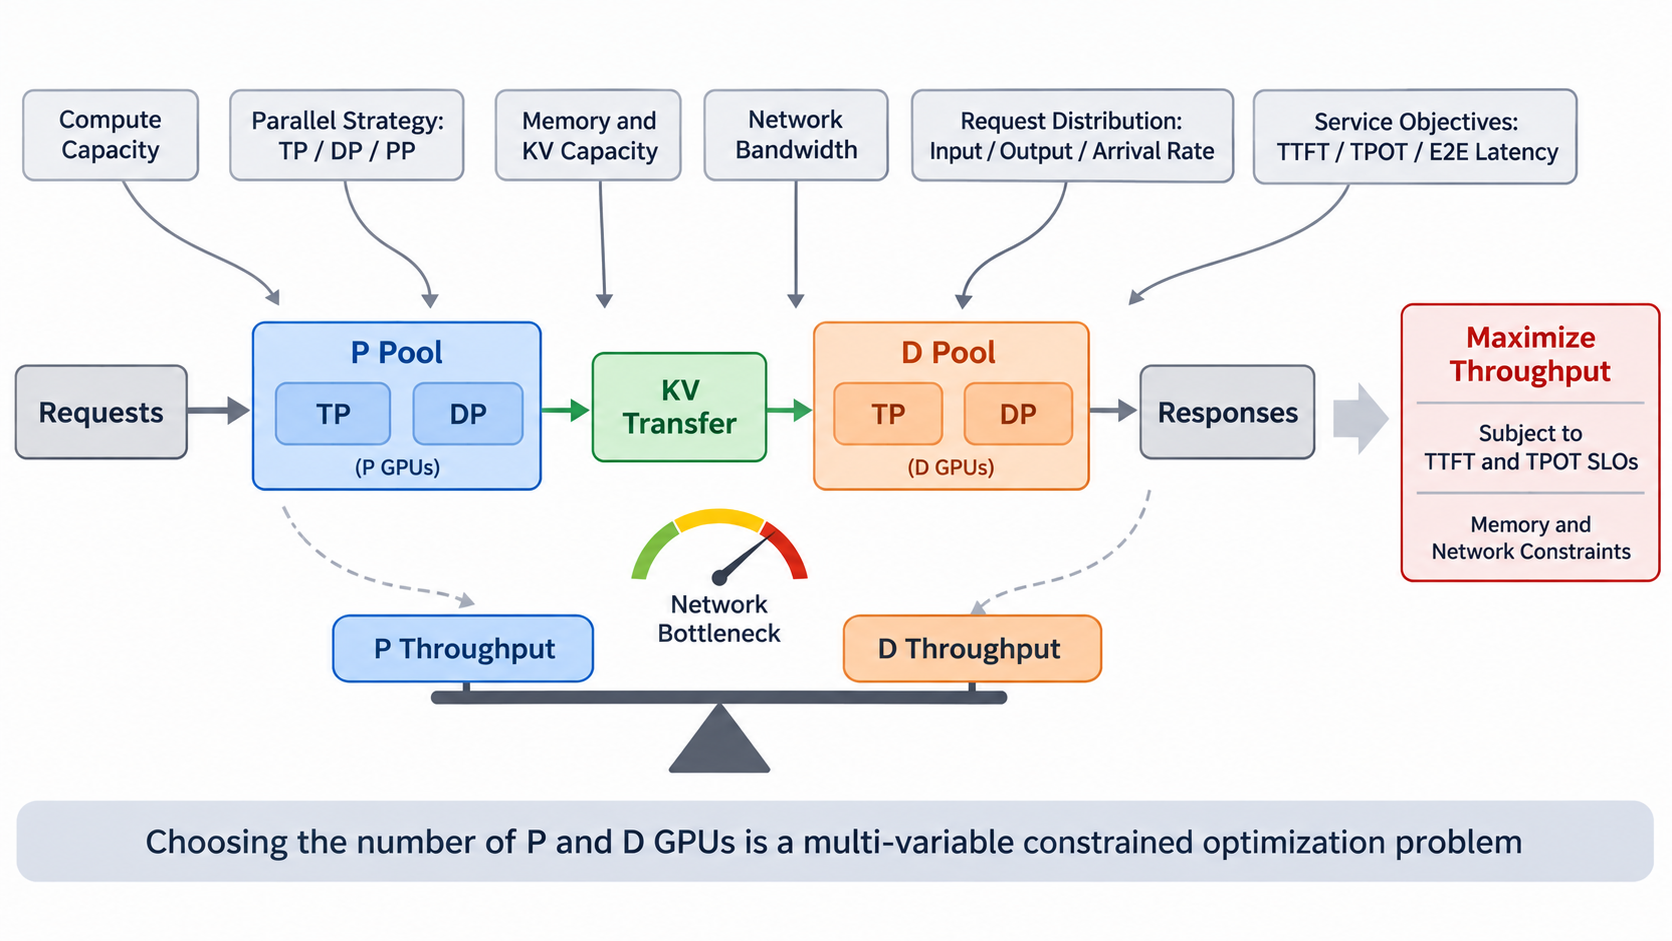
\includegraphics[width=0.9\textwidth]{fig-system.png}
  \caption{PD 分离需要同时满足吞吐、延迟 SLO 以及显存、带宽等资源约束}
  \label{fig:system}
\end{figure}

\textbf{PD 分离的本质，不是简单地把一个模型拆成两个阶段，而是将两种计算特征不同、资源需求不同的负载解耦，再通过合理的资源配置和调度策略，让整个推理系统达到更高的效率。}

\end{document}
